\documentclass[letterpaper,12pt]{formatfile}

% Packages
\usepackage[ruled]{algorithm2e}
\usepackage{amsfonts}
\usepackage{amsmath}
\usepackage{amssymb}
\usepackage{authblk}
\usepackage{bbm}
\usepackage{bbold}
\usepackage{bigints}
\usepackage{cancel}
\usepackage{character}
\usepackage[shortlabels]{enumitem}
\usepackage{float}
\usepackage[multiple]{footmisc}
\usepackage{fullpage}
\usepackage{gensymb}
\usepackage{graphicx}
\usepackage{hyperref}
\usepackage{mathtools}
\usepackage{mdframed}
\usepackage{multicol}
\usepackage[authoryear, round]{natbib}
\usepackage{subcaption}
\usepackage[numbib]{tocbibind}
\usepackage{xfrac}

%-----------------------------------------------------------------------%
% BEGIN DOCUMENT %
%-----------------------------------------------------------------------%
\begin{document}
\setlength{\fboxsep}{1.0mm}
\noindent

%-----------------------------------------------------------------------%
% TITLE %
%-----------------------------------------------------------------------%
\title{hashin\_shtrikman\_mp: a package for the optimal design and discovery of multi-phase composite materials}

\author[1]{Carla J. Becker}
\author[2,3]{Hrushikesh Sahasrabuddhe}
\author[2,4]{Max C. Gallant}
\author[3]{Anubhav Jain}
\author[2,4]{Kristin A. Persson}
\author[1]{Tarek I. Zohdi}

\affil[1]{Department of Mechanical Engineering, University of California, Berkeley, California, United States of America}
\affil[2]{Department of Materials Science and Engineering, University of California, Berkeley, California, United States of America}
\affil[3]{Energy Technologies Area, Lawrence Berkeley National Laboratory, Berkeley, CA 94720, USA}
\affil[4]{Materials Sciences Division, Lawrence Berkeley National Laboratory, Berkeley, California, United States of America}

\maketitle
  
%-----------------------------------------------------------------------%
% SUMMARY %
%-----------------------------------------------------------------------%
\section{Summary} \label{sec:summary}

\verb|hashin_shtrikman_mp| is a tool for composites designers who have desired composite properties in mind, but who do not yet have an underlying formulation. The library utilizes the tightest theoretical bounds on the effective properties of composite materials with unspecified microstructure – the Hashin-Shtrikman bounds – to identify candidate theoretical materials, find real materials that are close to the candidates, and determine the optimal volume fractions for each of the constituents in the resulting composite. Its i) leveraging of materials in the \href{https://next-gen.materialsproject.org/}{Materials Project} database, ii) integration with the \href{https://next-gen.materialsproject.org/api}{Materials Project API}, iii) use of genetic machine-learning and iv) agnosticism to underlying microstructure, and ultimate engineering application, make it a tool with much broader applications than its predecessors. 

%-----------------------------------------------------------------------%
% STATEMENT OF NEED %
%-----------------------------------------------------------------------%
\section{Statement of Need} \label{sec:need}

Composites are ubiquitous in engineering due to their tunability and enhanced material properties as compared to their individual constituents. As such, composite design is an active field, but the pursuit of new materials through experimentation is expensive. Today, computational tools for materials design are integral to reducing the cost and increasing the pace of innovation in the energy, electronics, aviation sectors, and beyond.

Several Python packages already exist for specific areas in composites modeling, such as \href{https://github.com/rafaelcidade/compositeslib}{CompositesLib}, \href{https://github.com/echaffey/Compysite}{Compysite}, \href{https://github.com/azzeddinetiba/FeCLAP}{FeCLAP}, and \href{https://pypi.org/project/material-mechanics/}{material-mechanics}, all of which perform stress analysis on laminates and/or fiber-reinforced composites using either classical laminate theory or the finite element method. Others exist which, like \verb|hashin_shtrikman_mp|, utilize the Hashin-Shtrikman bounds on effective composite properties, such as  \href{https://geodynamics.github.io/burnman/}{BurnMan} for thermal analysis of composite rocks/assemblages, \href{https://rockphypy.readthedocs.io/en/latest/getting_started/08_Shaly_sand_modelling.html}{rockphypy} for mechanical modeling of sand-shale systems, \citep{ZARE2017176}'s modeling of clay nanocomposites, and \citep{ZERHOUNI2019344}'s modeling of 3D printed microstructures. All of these tools, however, are highly specific to composite microstructure, macro-geometry, and composition. More notably, they focus on analysis of already well-defined composites, rather than discovery of new materials.

\verb|hashin_shtrikman_mp| is intended for composites designers who are much earlier in their design process -- designers who are seeking out new composite formulations and who are not yet tied to a specific underlying microstructure. \verb|hashin_shtrikman_mp| defines an inverse problem wherein composite formulations which achieve a desired behavior are found by minimizing a cost function \citep{zohdi2012electromagnetic}. Accounting for both absolute error from the desired properties and targeting even load distribution across constituent phases, \verb|hashin_shtrikman_mp| returns candidate theoretical materials, then searches for real materials in the Materials Project database with properties close to the recommended constituents. 

%-----------------------------------------------------------------------%
% UNDERLYING THEORY
%-----------------------------------------------------------------------%
\section{Underlying Theory} \label{sec:theory}

%%%%%%%%%%%%%%%%%%%%%%%%%%%%%%%%%%%%%%%%%%%%%%%%%%%%%%%%%
% Hashin-Shtrikman Bounds on Composite Properties
%%%%%%%%%%%%%%%%%%%%%%%%%%%%%%%%%%%%%%%%%%%%%%%%%%%%%%%%%
\subsection{Estimate effective composite properties with the Hashin-Shtrikman bounds} \label{subsec:HS-bounds}
When designing composites, simple volume-weighted linear combinations of constituent material properties do not yield accurate approximations of the resulting effective composite properties. Instead, for laminates, materials designers often bound the resulting composite properties using equations from constitutive elastic theory, such as the Hill-Reuss-Voight-Weiner bounds, where the lower bound is the harmonic mean of the constituent material properties and the upper bound is the arithmetic mean \citep{commentaryHS}. For quasi-isotropic and quasi-homogeneous multi-phase composites with arbitrary phase geometry (a more general case), a better option is to use the Hashin-Shtrikman bounds, which provide even tighter ranges on the resulting effective properties \citep{hashin1962variational}. Equation \ref{eqn:gen_ineq} summarizes the Hashin-Shtrikman bounds on a generalized effective material property $y^{*}$ of an $n$-phase composite. The generalized material properties for the $n$-phases are ordered from least to greatest where $y_{1} \leq y_{2} \leq \dotsb \leq y_{n}$ with corresponding volume fractions sum to unity $v_{1} + v_{2} + \dotsb + v_{n} = 1$:

\begin{equation}
y_{1} + \frac{A_{1}}{1 - \alpha_{1}A_{1}}
= y^{*,-} \leq y^{*} \leq y^{*,+} = 
y_{n} + \frac{A_{n}}{1 - \alpha_{n}A_{n}}
\label{eqn:gen_ineq}
\end{equation}

\noindent where
\begin{equation}
\alpha_{1} = \frac{1}{3y_{1}}
\quad \text{and} \quad
\alpha_{n} = \frac{1}{3y_{n}},
\label{eqn:gen_alphas}
\end{equation}

\noindent and
\begin{equation}
A_{1} = \sum\limits_{i=2}^{n} \frac{v_{i}}{\frac{1}{y_{i} - y_{1}} + \alpha_{1}}
\quad \text{and} \quad
A_{n} = \sum\limits_{i=1}^{n-1} \frac{v_{i}}{\frac{1}{y_{i} - y_{n}} + \alpha_{n}}.
\label{eqn:gen_As}
\end{equation}


\begin{figure}
    \centering
    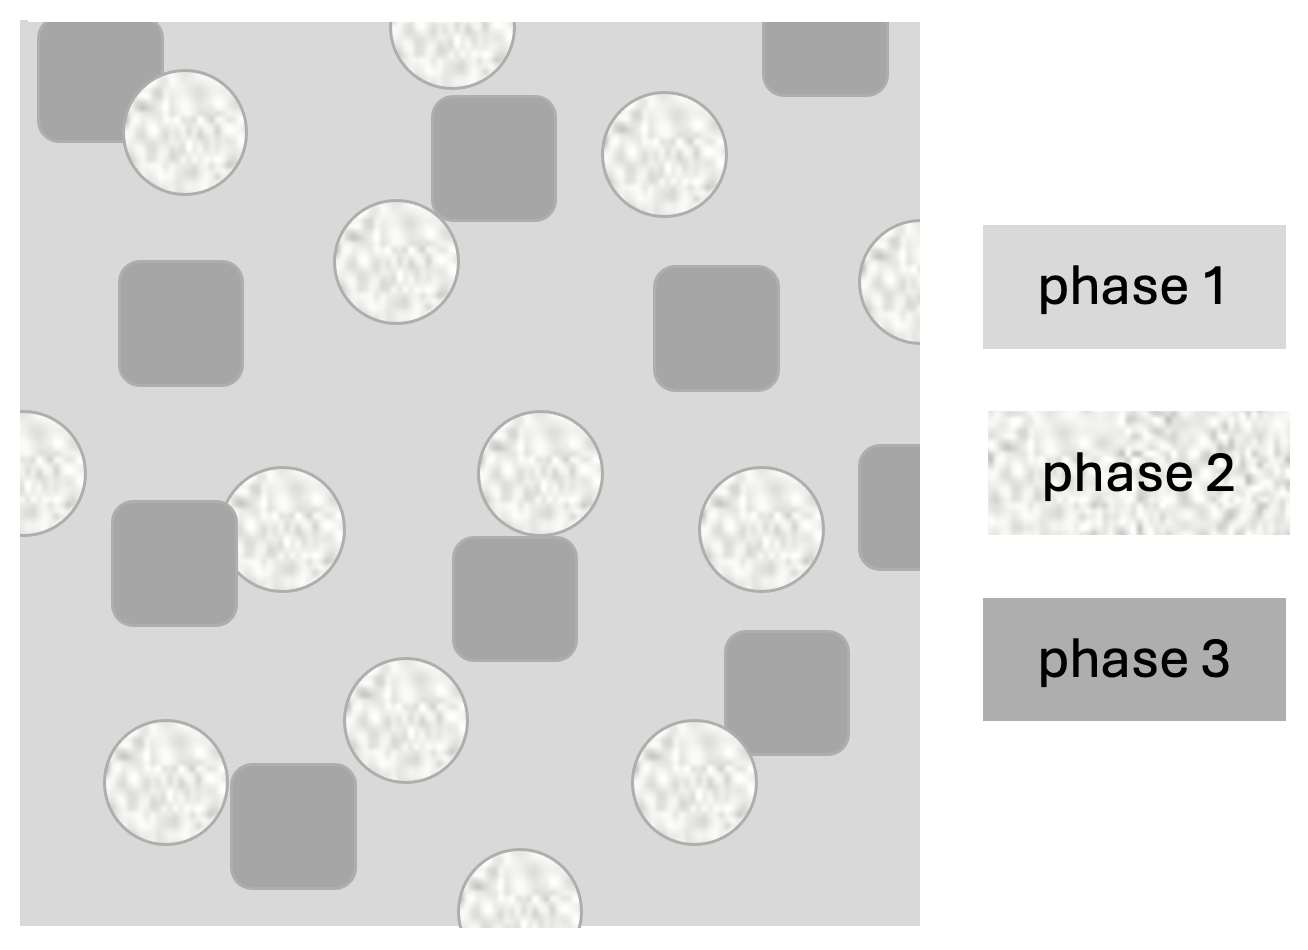
\includegraphics[width=2in]{figures/3phase_composite.png}
    \caption{An example of a quasi-isotropic, quasi-homogeneous 3-phase composite.}
    \label{fig:cartoon-3phase}
\end{figure}

Equations \ref{eqn:bulk_ineq} and \ref{eqn:shear_ineq} summarize the results of the Hashin-Shtrikman derivations on the bounds on effective bulk modulus $\kappa^{*}$ and effective shear modulus $\mu^{*}$, where we simultaneously require $\kappa_{1} \leq \kappa_{2} \leq \dotsb \leq \kappa_{n}$ and $\mu_{1} \leq \mu_{2} \leq \dotsb \leq \mu_{n}$:

\begin{equation}
\kappa_{1} + \frac{A_{1}^{\kappa}}{1 - \alpha_{1}^{\kappa}A_{1}^{\kappa}}
= \kappa^{*,-} \leq \kappa^{*} \leq \kappa^{*,-} = 
\kappa_{n} + \frac{A_{n}^{\kappa}}{1 - \alpha_{n}^{\kappa}A_{n}^{\kappa}}
\label{eqn:bulk_ineq}
\end{equation}

\begin{equation}
\mu_{1} + \frac{A_{1}^{\mu}}{1 - \alpha_{1}^{\mu}A_{1}^{\mu}}
= \mu^{*,-} \leq \mu^{*} \leq \mu^{*,-} = 
\mu_{n} + \frac{A_{n}^{\mu}}{1 - \alpha_{n}^{\mu}A_{n}^{\mu}}
\label{eqn:shear_ineq}
\end{equation}

\noindent with
\begin{equation}
\alpha_{1}^{\kappa} = \frac{3}{3\kappa_{1} + 4\mu_{1}}
\quad \text{and} \quad
\alpha_{n}^{\kappa} = \frac{3}{3\kappa_{n} + 4\mu_{n}},
\label{eqn:bulk_alphas}
\end{equation}

\noindent and
\begin{equation}
\alpha_{1}^{\mu} = \frac{3(\kappa_{1} + \mu_{1})}{5\mu_{1}(3\kappa_{1} + 4\mu_{1})}
\quad \text{and} \quad
\alpha_{n}^{\mu} = \frac{3(\kappa_{n} + \mu_{n})}{5\mu_{n}(3\kappa_{n} + 4\mu_{n})},
\label{eqn:shear_alphas}
\end{equation}

\noindent and
\begin{equation}
A_{1}^{\kappa} = \sum\limits_{i=2}^{n} \frac{v_{i}}{\frac{1}{\kappa_{i} - \kappa_{1}} + \alpha_{1}}
\quad \text{and} \quad
A_{n}^{\kappa} = \sum\limits_{i=1}^{n-1} \frac{v_{i}}{\frac{1}{\kappa_{i} - \kappa_{n}} + \alpha_{n}}, 
\label{eqn:bulk_As}
\end{equation}

\noindent and
\begin{equation}
A_{1}^{\mu} = \sum\limits_{i=2}^{n} \frac{v_{i}}{\frac{1}{\kappa_{i} - \kappa_{1}} + \alpha_{1}}
\quad \text{and} \quad
A_{n}^{\mu} = \sum\limits_{i=1}^{n-1} \frac{v_{i}}{\frac{1}{\mu_{i} - \mu_{n}} + \alpha_{n}}.
\label{eqn:shear_As}
\end{equation}

\noindent The elastic forms for $\{A_{i}^{\kappa}\}$ and $\{A_{i}^{\mu}\}$ differ from the general forms $\{A_{i}\}$ because of their coupling via the Kirchoff-St. Venant constitutive law.

Once upper and lower bounds on the effective composite properties have been obtained, what remains is to find a final estimate of the resulting material properties. By the definition of bounds, we can write an expression for the effective property as
\begin{equation}
y^{*} = \gamma y^{*,-} + (1-\gamma) y^{*,+}.
\label{eqn:mixing-param}
\end{equation}

\noindent Given experimental data we could fit $\gamma$ and extrapolate for a range of volume fractions, but, in the absence of experimental data, we select $\gamma = 0.5$. For more information, the reader is referred to \cite{zohdi-course-reader}.

%%%%%%%%%%%%%%%%%%%%%%%%%%%%%%%%%%%%%%%%%%%%%%%%%%%%%%%%%
% Concentration Tensors and Quantifying Distributed Load
%%%%%%%%%%%%%%%%%%%%%%%%%%%%%%%%%%%%%%%%%%%%%%%%%%%%%%%%%
\subsection{Quantifying distributed loads with concentration tensors} \label{subsec:conc-facs}
In addition to finding effective properties of potential composites, \verb|hashin_shtrikman_mp| recommends composites that are less prone to failure under extreme loading. When loads are not efficiently shared between constituents of the composite, stress concentrations, hot spots, and electrical shorts can develop, eventually leading to material failure. By introducing the concept of ``concentration tensors", we can quantify a constituent's contribution to load response and then use constitutive laws to determine how the composite will respond to loads. 

For the general case of a constitutive law of the form
\begin{equation}
\verb|tensor-valued response| = \verb|proportionality tensor| \times \verb|tensor-valued load|,
\label{eqn:gen-const-law}
\end{equation}

\noindent over the domain $\Omega$, we note that, by the definition of volume fraction, the following holds:
\begin{equation}
\langle \verb|tensor-valued load| \rangle_{\Omega} = \sum\limits_{i=1}^{n} v_{i} \langle \verb|tensor-valued load| \rangle_{\Omega_{i}} \\[15pt]
\label{eqn:by-vol-frac-load}
\end{equation}

\noindent and
\begin{equation}
\langle \verb|tensor-valued response| \rangle_{\Omega} = \sum\limits_{i=1}^{n} v_{i} \langle \verb|tensor-valued response| \rangle_{\Omega_{i}},
\label{eqn:by-vol-frac-resp}
\end{equation}

\noindent where $\langle \cdot \rangle_{\Omega} = \frac{1}{|\Omega|} \int_{\Omega} (\cdot) \,d\Omega$ is the average of $(\cdot)$ over the domain, $v_{i}$ is the volume fraction of phase $i$, and $n$ is the number of phases. From there, we define the concentration tensors for the applied loads and responses for phases $i\in[1,...,n]$, respectively, as
\begin{equation}
\langle \verb|tensor-valued load| \rangle_{\Omega_{i}} \equiv C_{i, \text{load}} \langle \verb|tensor-valued load| \rangle_{\Omega} \\[15pt]
\label{eqn:Cload-basic-def}
\end{equation}

\noindent and
\begin{equation}
\langle \verb|tensor-valued response| \rangle_{\Omega_{i}} \equiv C_{i, \text{response}} \langle \verb|tensor-valued response| \rangle_{\Omega}.
\label{eqn:Cresp-basic-def}
\end{equation}

\noindent It follows from these definitions, and the assumption that the composite is isotropic and homogeneous, that the concentration tensors can be written only in terms of proportionality tensors. The concentration tensors for the applied loads for phases $i\in[2,...,n]$ are subsequently given by
\begin{equation}
\begin{array}{l}
\bC_{i,\text{load}} = \displaystyle\frac{1}{n-1} \displaystyle\frac{1}{v_{i}} \times \\[10pt]
\hspace{16mm} [(\text{effective } \texttt{proportionality tensor}) - (\text{phase $i$ }\texttt{proportionality tensor})]: \\[10pt]
\hspace{20mm} [(\text{phase $i$ }\texttt{proportionality tensor}) - (\text{phase 1 }\texttt{proportionality tensor})]^{-1}
\end{array}
\label{eqn:load-conc-fact}
\end{equation}

\noindent and for phase 1 as
\begin{equation}
\bC_{1,\text{load}} = \frac{1}{v_{1}} \left( 1 - \sum\limits_{i=2}^{n} v_{i} \bC_{i,\text{load}} \right),
\label{eqn:C1load}
\end{equation}

\noindent The concentration tensors for the responses for phases $i\in[2,...,n]$ are given by 
\begin{equation}
\bC_{i,\text{response}} = (\text{phase $i$ } \verb|proportionality tensor|)\bC_{i,\text{load}}(\text{effective } \verb|proportionality tensor|)^{-1}
\label{eqn:response-conc-fact}
\end{equation}

\noindent and for phase 1 as
\begin{equation}
\bC_{1,\text{response}} = \frac{1}{v_{1}} \left( 1 - \sum\limits_{i=2}^{n} v_{i} \bC_{i,\text{response}} \right).
\label{eqn:C1response}
\end{equation}

As a concrete example, consider Ohm's law, which relates the applied electric field $\bE$ (load) to the resulting current density $\bJ$ (response) via the electrical conductivity $\Bsigma_{e}$ (proportionality tensor), governing a 3-phase composite. The concentration tensors for current density would be
\begin{equation}
\begin{array}{l}
\bC_{1,J} = \displaystyle\frac{1}{v_{1}} \left( 1 - v_{2} \bC_{2,J} - v_{3} \bC_{3,J} \right), \\[10pt]
\bC_{2,J} = \Bsigma_{2,e}:\bC_{2,E}:(\Bsigma_{e}^{*})^{-1}, \\[10pt]
\bC_{3,J} = \Bsigma_{3,e}:\bC_{3,E}:(\Bsigma_{e}^{*})^{-1},
\end{array}
\label{eqn:J_cfs}
\end{equation}

\noindent where $\Bsigma_{e}^{*}$ would be found according to the previous section. The concentration tensors for electric field would be
\begin{equation}
\begin{array}{l}
\bC_{1,E} = \displaystyle\frac{1}{v_{1}} \left( 1 - v_{2} \bC_{2,E} - v_{3} \bC_{3,E} \right), \\[10pt]
\bC_{2,E} = \displaystyle\frac{1}{2}\displaystyle\frac{1}{v_{2}} (\Bsigma_{e}^{*} - \Bsigma_{1,e}):(\Bsigma_{2,e}^{*} - \Bsigma_{1,e})^{-1}, \\[10pt]
\bC_{3,E} = \displaystyle\frac{1}{2}\displaystyle\frac{1}{v_{3}} (\Bsigma_{e}^{*} - \Bsigma_{1,e}):(\Bsigma_{3,e}^{*} - \Bsigma_{1,e})^{-1}.
\end{array}
\label{eqn:E_cfs}
\end{equation}

In the case where the constitutive law governing concentration tensors is the Kirchoff-St. Venant law, which relates the tensor-valued strain to the tensor-valued stress via the tensor-valued stiffness, we can additionally define scalar-valued concentration factors $C_{i,\kappa}$ and $C_{i,\mu}$, which respectively are the concentration factors for hydrostatic and deviatoric stress. For phases $i\in[2,...,n]$ They are defined as
\begin{equation}
C_{i,\kappa} = \frac{1}{v_{i}}\frac{\kappa_{i}}{\kappa^{*}}(\kappa^{*} - \kappa_{1})(\kappa_{i} - \kappa_{1})^{-1}
\label{eqn:sph-conc-fact}
\end{equation}

\noindent and
\begin{equation}
C_{i,\mu} = \frac{1}{v_{i}}\frac{\mu_{i}}{\mu^{*}}(\mu^{*} - \mu_{1})(\mu_{i} - \mu_{1})^{-1},
\label{eqn:dev-conc-fact}
\end{equation}

\noindent where 
\begin{equation}
\left\langle \frac{1}{3}\text{tr}\Bsigma \right\rangle_{\Omega_{i}} \equiv C_{i,\kappa} \left\langle \frac{1}{3}\text{tr}\Bsigma \right\rangle_{\Omega} 
\label{eqn:sph-conc-fact-def}
\end{equation}

\noindent and
\begin{equation}
\left\langle \Bsigma' \right\rangle_{\Omega_{i}} \equiv C_{i,\kappa} \left\langle \Bsigma' \right\rangle_{\Omega}.
\label{eqn:dev-conc-fact-def}
\end{equation}

\noindent For phase 1, the concentration tensors are defined as
\begin{equation}
C_{1,\kappa} = \frac{1}{v_{1}} \left( 1 - \sum\limits_{i=2}^{n} v_{i} C_{i,\kappa} \right)
\label{eqn:sph-cf-1}
\end{equation}

\noindent and
\begin{equation}
C_{1,\mu} = \frac{1}{v_{1}} \left( 1 - \sum\limits_{i=2}^{n} v_{i} C_{i,\mu} \right).
\label{eqn:dev-cf-1}
\end{equation}

\noindent For more information, the reader is referred to \cite{zohdi-course-reader}.

%-----------------------------------------------------------------------%
% PACKAGE OVERVIEW %
%-----------------------------------------------------------------------%
\section{Package Overview} \label{sec:package-overview}

%-----------------------------------------------------------------------%
% Implementation Notes %
%-----------------------------------------------------------------------%
\subsection{Implementation Notes} \label{subsec:implementation}
The library has been designed to handle the design of 2- to 10-phase isotropic and homogeneous composites. All materials in the Materials Project database are available for search through \verb|hashin_shtrikman_mp|, but it is recommended that users restrict the search bounds for universal anisotropy to be between 0.5 and 1.5 for results closer to theory. Additionally, at the time of this writing, because of the assumption that the composite and its constituents are isotropic and homogeneous, the full tensor forms for the effective properties and concentration tensors are collapsed to scalar forms. This is simpler computationally and allows the same code to be used for all properties (aside from bulk and shear moduli, which cannot be decoupled). For material properties in the Materials Project database with full tensor values available, \verb|hashin_shtrikman_mp| uses the largest eigenvalue. Figure \ref{fig:flow-chart} is a flow chart demonstrating the most common usage of \verb|hashin_shtrikman_mp|.

\pagebreak
\begin{figure}[H]
    \centering
    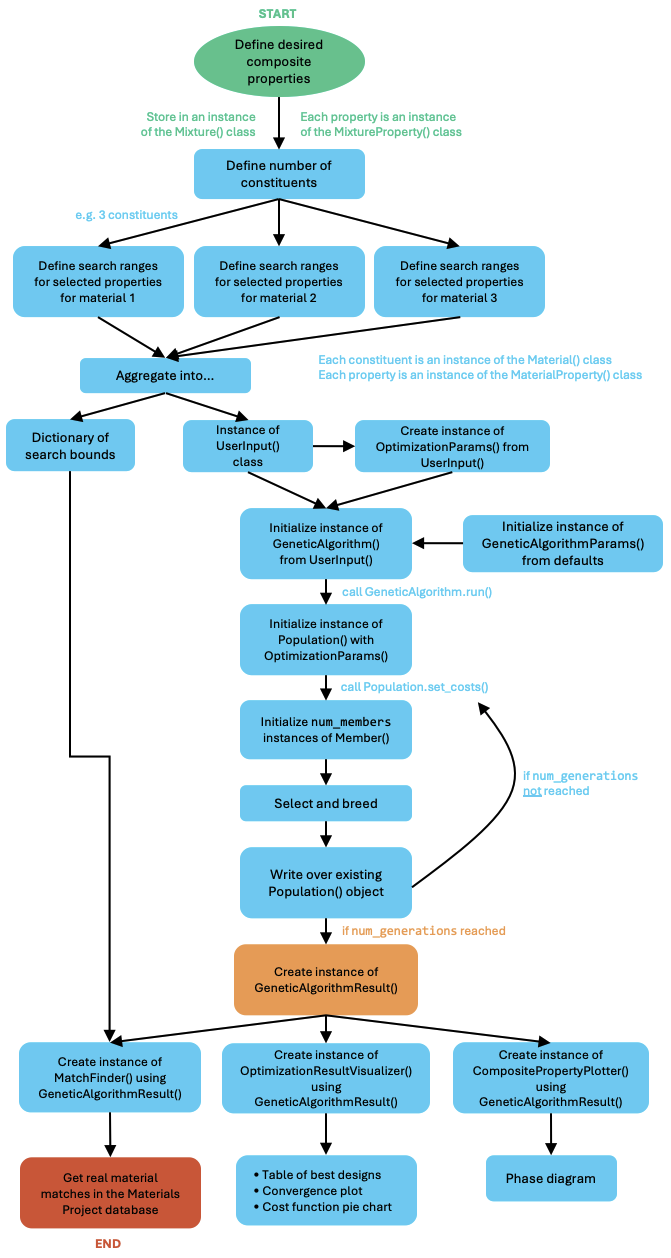
\includegraphics[height=9in]{figures/hashin_shtrikman_mp_flow_chart.png}
    \caption{A flow chart demonstrating the most common usage of $\texttt{hashin\_shtrikman\_mp}$.}
    \label{fig:flow-chart}
\end{figure}

%-----------------------------------------------------------------------%
% Cost function design and optimization with genetic algorithm %
%-----------------------------------------------------------------------%
\subsection{Cost function design and optimization with genetic algorithm} \label{subsec:GA}
To find optimal composite mixtures, \verb|hashin_shtrikman_mp| simultaneously seeks composite compositions with effective properties close to the desired properties and seeks to ensure even load sharing among the composite constituent phases. Accordingly, the cost function is constructed in the following way. 

Each property category selected by a user contributes its own term to the total cost function. At the time of this writing, the possible property categories are elastic, dielectric, carrier-transport, magnetic, and piezoelectric. Combining the individual cost functions to optimize across all design goals simultaneously yields 
\begin{equation}
\Pi^{\text{total}} = W_{\text{domains}}\left[ \Pi^{\text{elastic}} + \Pi^{\text{dielectric}} + \Pi^{\text{carrier-transport}} + \Pi^{\text{magnetic}} + \Pi^{\text{piezoelectric}} \right]
\label{eqn:pi}
\end{equation}

\noindent where $W_{\text{domains}}$ normalizes for the number of active property categories. Each property category contribution is composed of two weighted sums: 1) one with terms for absolute error between the effective and desired properties and 2) another for the absolute error between the concentration factors and a tolerance \verb|TOL| that quantifies ``well-distributed" load sharing. That is,
\begin{equation}
\Pi^{\text{general}} =
\begin{cases}
\begin{array}{l}
w_{\text{eff}} \sum\limits_{i=1}^{n_{\text{props}}} \biggl\vert\displaystyle\frac{y_{i}^{*,D} - y_{i}^{*}}{y^{*,D}}\biggr\vert 
+ \sum\limits_{i=1}^{n_{\text{cfs}}} \hat{w}_{\text{cf}}^{i} \biggl\vert\displaystyle\frac{C_{i}-\texttt{TOL}}{\texttt{TOL}}\biggr\vert,
\end{array} & \text{if property category active}, \\
\hspace{3mm} 0, & \text{else},
\end{cases}
\label{eqn:pi-gen}
\end{equation}

\noindent where the superscript $D$ denotes the desired value, $n_{\text{props}}$ is the number of properties in that property category, $n_{\text{cfs}}$ is the number of concentration factors in that category (typically two $\times$ the number of properties), and $C_{i}$ is a general scalar-valued concentration factor from section \ref{sec:theory}\ref{subsec:conc-facs}. Note also that $w_{\text{eff}} = 1/n_{\text{props}}$ and

\begin{equation}
\hat{w}_{\text{cf}}^{i} = 
\begin{cases}
w_{\text{cf}}, & C_{i} >  \texttt{TOL}, \\
0, & \text{otherwise},
\end{cases}
\end{equation}

\noindent where $w_{\text{cfs}} = 1/(2n_{\text{props}}n_{\text{materials}})$, except in the elastic case where $w_{\text{cfs}} = 1/n_{\text{props}}n_{\text{materials}}$.

As a concrete example, the dielectric contribution to the cost function would take the form
\begin{equation}
\Pi^{\text{dielectric}} =
\begin{cases}
\begin{array}{l}
w_{\text{eff}} \biggl\vert\displaystyle\frac{\epsilon^{*,D} - \epsilon^{*}}{\epsilon_{ij}^{*,D}}\biggr\vert \\[10pt]
\hspace{3mm} + \hat{w}_{\text{cf}}^{i, E} \biggl\vert\displaystyle\frac{C_{i,E}-\texttt{TOL}}{\texttt{TOL}}\biggr\vert, 
+ \hat{w}_{\text{cf}}^{i, E_{0}} \biggl\vert\displaystyle\frac{C_{i,E_{0}}-\texttt{TOL}}{\texttt{TOL}}\biggr\vert,
\end{array} & \text{if dielectric property category active}, \\
\hspace{3mm} 0, & \text{else},
\end{cases}
\label{eqn:pi-elastic}
\end{equation}

\noindent where the constitutive law, in the scalar case, relates applied field $E_{0}$ to resulting field $E$ via the dielectric constant $\epsilon$ according to $E = \epsilon E_{0}$ and the same rules for the weights apply as above.  

With the cost function defined, \verb|hashin_shtrikman_mp| converges to an optimal solution with a genetic algorithm. Each member of a population in the genetic algorithm is composed of candidate material property values. After successive selection and breeding over many generations, the genetic algorithm will converge. The default genetic algorithm parameters are 10 parents, 10 children, 200 members per population, and 100 generations, but a user can change them. Given the cost function design, the cost value can be thought of as the fractional error from the desired outcome, plus penalties for ``bad" load sharing (should contribute 0 in the case of ``good" load sharing). A user can monitor the results of the genetic algorithm with the convergence plot, included in Figure \ref{fig:convg}. 

The nature of genetic algorithms is to produce several offspring with the same properties and costs after many generations, thus \verb|hashin_shtrikman_mp| presents the user with only the \textit{unique} top performing designs in a table. For the singular lowest-cost performer, users are presented with a breakdown of the cost, as in Figure \ref{fig:cost-func-contribs}.

%-----------------------------------------------------------------------%
% Visualization and analysis %
%-----------------------------------------------------------------------%
\subsection{Visualization and analysis} \label{subsec:viz}
\verb|hashin_shtrikman_mp| provides visualization tools for the genetic algorithm results and for matches with 2-, 3-, or 4- phases. 

Figure \ref{fig:convg} is a convergence plot showing the value of the genetic algorithm cost function decreasing over generations. The monotonically decreasing, staircase nature is characteristic to genetic algorithm convergence, where the best performer may remain the best for several generations and where several genetic strings may converge to the same value (e.g. when average cost of top ten performers equals the best cost). As the cost function has been designed to represent absolute error from the desired properties, a cost of 1.0 represents 100\% error. 

Figure \ref{fig:cost-func-contribs} contains a breakdown of the non-zero cost at the end of optimization for a 3-phase material where the properties of interest were electrical conductivity, thermal conductivity, bulk modulus, shear modulus, and universal anisotropy. We expect the cost function to have 31 terms in this case, as there is one effective property term per property and there are two concentration factor terms per property per material, except in the coupled case of bulk and shear moduli, where there are two concentration factors per material instead of the expected four i.e.
\begin{itemize}
\item 5 effective properties: one for each of the properties of interest,
\item 18 non-modulus concentration factors: one load and one response concentration factor for each of the 3 non-elastic properties (electrical conductivity, thermal conductivity, and universal anisotropy), and for each of the 3 phases, and
\item 6 modulus concentration factors: one hydrostatic and one deviatoric concentration factor for each of the 3 phases.
\end{itemize}

\begin{figure}[H]
    \centering
        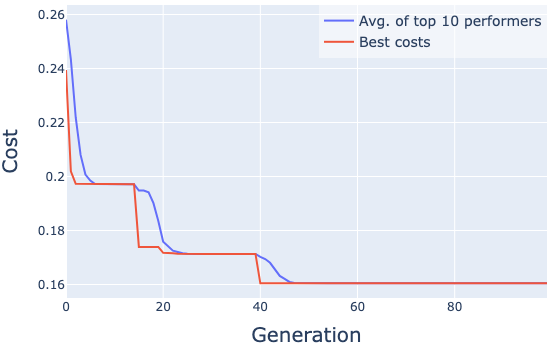
\includegraphics[width=0.6\textwidth]{figures/convg.png}
        \caption{An example of the convergence plot for the genetic algorithm.}
        \label{fig:convg}
\end{figure}

\begin{figure}[H]
    \centering
        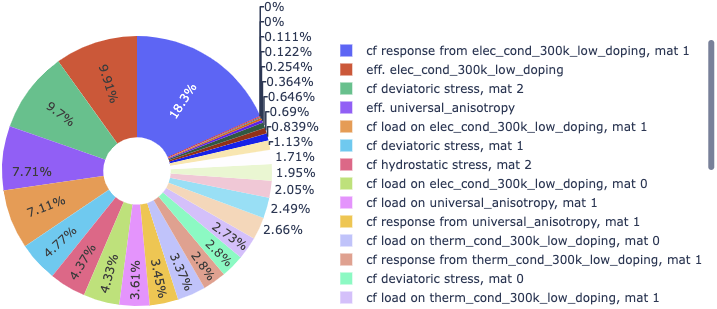
\includegraphics[width=0.9\textwidth]{figures/cost-func-contribs.png}
        \caption{A breakdown of the contributions to the non-zero cost at the end of optimization.}
        \label{fig:cost-func-contribs}
\end{figure}

Once matches have been identified for a desired composite, along with recommended volume fractions, a user can still explore how varying the volume fractions of the constituents affect the resulting effective properties through interactive phase diagrams. Examples of these phase diagrams are included in Figure \ref{fig:phase-viz}.

\begin{figure}[H]
    \centering
    % Top row
    \begin{subfigure}[t]{0.4\textwidth}
        \centering
        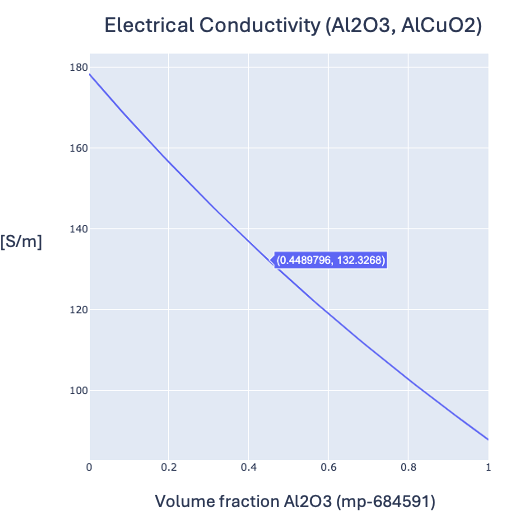
\includegraphics[width=\textwidth]{figures/elec-cond-2phase-clean.png}
        \caption{}
        \label{fig:2phase}
    \end{subfigure}
    \hfill
    \begin{subfigure}[t]{0.5\textwidth}
        \centering
        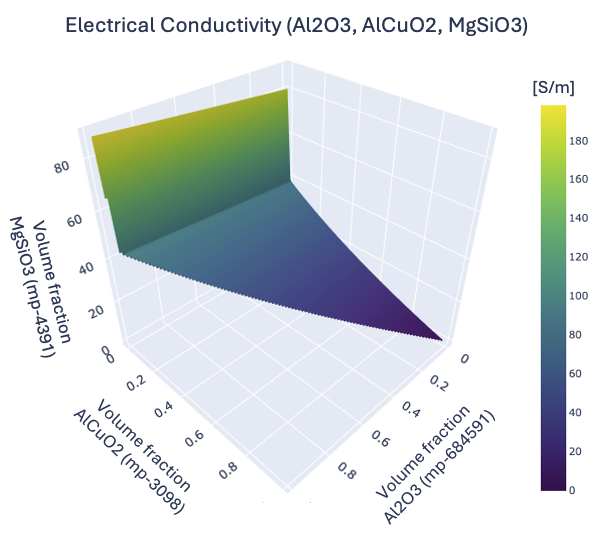
\includegraphics[width=\textwidth]{figures/elec-cond-3phase-clean.png}
        \caption{}
        \label{fig:3phase}
    \end{subfigure}

    % Bottom row
    \begin{subfigure}[t]{0.5\textwidth}
        \centering
        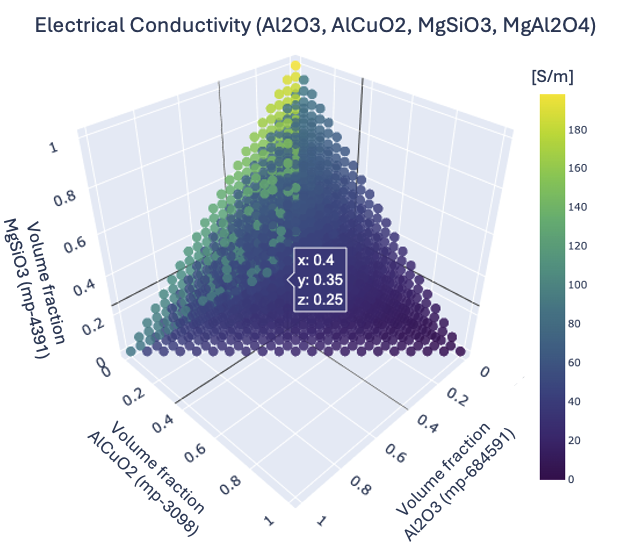
\includegraphics[width=\textwidth]{figures/elec-cond-4phase-clean.png}
        \caption{}
        \label{fig:4phase}
    \end{subfigure}

    \caption{Example phase diagrams for 2-, 3-, and 4-phase mixtures of Al\textsubscript{2}O\textsubscript{3} (mp-684591), AlCuO\textsubscript{2} (mp-3098), MgSiO\textsubscript{3} (mp-4391), and MgAl\textsubscript{2}O\textsubscript{4} (mp-3536).}
    \label{fig:phase-viz}
\end{figure}

%-----------------------------------------------------------------------%
% Match-finding %
%-----------------------------------------------------------------------%
\subsection{Match-finding} \label{subsec:match-finding}

The genetic algorithm returns suggested material properties for each of the phases in the composite and then \verb|hashin_shtrikman_mp| finds real materials in the Materials Project database which are similar, according to some percent error threshold, which the user can control.

%-----------------------------------------------------------------------%
% ACKNOWLEDGMENTS %
%-----------------------------------------------------------------------%
\section{Acknowledgments} \label{sec:ack}
This work was primarily funded by the Materials Project, which is funded by the U.S. Department of Energy, Office of Science, Office of Basic Energy Sciences, Materials Sciences and Engineering Division, under Contract no. DE-AC02-05-CH11231: Materials Project program KC23MP. The project has been intellectually led by Tarek Zohdi and Kristin Persson. We would also like to thank the software engineering team at the Materials Project -- Patrick Huck, Jason Munro, and Ruoxi Yang  -- for their support.

%-----------------------------------------------------------------------%
% REFERENCES %
%-----------------------------------------------------------------------%
\bibliographystyle{plainnat}
\bibliography{Refs}
\end{document} 
